% questions.tex —— 2016 年·天津卷·文科 · 题目内容片段（无答案）
% 由 tools/generate_projects.py 依来源总账自 2016/2016_数学真题_天津文_试题.md 生成，勿手改（改源 MD 后重跑）


\gkpart{数学}

\begin{gktip}
\textbf{来源说明}：本题面依据固定源 PDF 两页 A3 页面逐题核对，原卷印刷页码 1025–1026。固定源不附答案；本文件仅为题面规范源。
\end{gktip}

\gkpart{一、选择题}

\begin{question}
\gkti{1}已知集合 \(A=\{1,2,3\}\)，\(B=\{y\mid y=2x-1,x\in A\}\)，则 \(A\cap B=\)（　）

\begin{gkopts}(2)
\task （A）\(\{1,3\}\)
\task （B）\(\{1,2\}\)
\task （C）\(\{2,3\}\)
\task （D）\(\{1,2,3\}\)
\end{gkopts}

\end{question}
\begin{question}
\gkti{2}甲、乙两人下棋，两人下成和棋的概率是 \(\dfrac{1}{2}\)，甲获胜的概率是 \(\dfrac{1}{3}\)，则甲不输的概率为（　）

\begin{gkopts}(2)
\task （A）\(\dfrac{5}{6}\)
\task （B）\(\dfrac{2}{5}\)
\task （C）\(\dfrac{1}{6}\)
\task （D）\(\dfrac{1}{3}\)
\end{gkopts}

\Needspace{0.4\textheight}
\end{question}
\begin{question}
\gkti{3}将一个长方形沿相邻三个面的对角线截去一个棱锥，得到的几何体的正视图与俯视图如图所示，则该几何体的侧（左）视图为（　）
\nopagebreak[4]
\begin{center}% 第 3 题三视图选择题题图组：2 个已知视图（正视图、俯视图，纵向叠放）+ 4 个选项侧（左）视图（横向排开）。
% 按固定源 PDF 矢量路径换算（1 pt → 0.03515 cm）；原点取图组左下（源页 (67.40, 566.30) pt），y 向上。
% 几何：俯视图为正方形 45.34×45.34 pt，其余为 1:2 竖长方形 45.34×90.67 pt（= 深 × 高）；两已知视图对角线均实线
% （正视图左上→右下、俯视图左下→右上）；选项 (A) 实线、(B) 虚线（均左上→右下），(C) 实线、(D) 虚线（均左下→右上）。
% 全组无尺寸标注；选项字母 (A)–(D) 在各选项图的左下方、图的左边缘之外（不在图下居中）。
\begin{tikzpicture}[line cap=round,line join=round,font=\small,x=0.03515cm,y=0.03515cm]
% ===== 已知视图 =====
% 正视图（竖长方形，实线对角线左上→右下）
\draw (133.30,186.28) rectangle (178.64,276.95);
\draw (133.30,276.95)--(178.64,186.28);
\node[anchor=base west,inner sep=0] at (140.22,171.76) {正视图};
% 俯视图（正方形，实线对角线左下→右上）
\draw (133.30,118.27) rectangle (178.64,163.61);
\draw (133.30,118.27)--(178.64,163.61);
\node[anchor=base west,inner sep=0] at (140.22,103.82) {俯视图};
% ===== 选项图（四个等大竖长方形，上下边齐平）=====
\draw (19.73,3.23) rectangle (65.07,93.91);
\draw (19.73,93.91)--(65.07,3.23);
\draw (104.30,3.23) rectangle (149.64,93.91);
\draw[dash pattern=on 2.99pt off 2.99pt] (104.30,93.91)--(149.64,3.23);
\draw (189.46,3.23) rectangle (234.79,93.91);
\draw (189.46,3.23)--(234.79,93.91);
\draw (274.90,3.23) rectangle (320.24,93.91);
\draw[dash pattern=on 2.99pt off 2.99pt] (274.90,3.23)--(320.24,93.91);
% 选项字母（图外左下）
\node[anchor=base west,inner sep=0] at (0,3.03) {(A)};
\node[anchor=base west,inner sep=0] at (85.01,3.03) {(B)};
\node[anchor=base west,inner sep=0] at (170.02,3.03) {(C)};
\node[anchor=base west,inner sep=0] at (255.02,3.03) {(D)};
\end{tikzpicture}
\end{center}
\nopagebreak[4]
\end{question}
\begin{question}
\gkti{4}已知双曲线 \(\dfrac{x^{2}}{a^{2}}-\dfrac{y^{2}}{b^{2}}=1\)（\(a>0\)，\(b>0\)）的焦距为 \(2\sqrt{5}\)，且双曲线的一条渐近线与直线 \(2x+y=0\) 垂直，则双曲线的方程为（　）

\begin{gkopts}(1)
\task （A）\(\dfrac{x^{2}}{4}-y^{2}=1\)
\task （B）\(x^{2}-\dfrac{y^{2}}{4}=1\)
\task （C）\(\dfrac{3x^{2}}{20}-\dfrac{3y^{2}}{5}=1\)
\task （D）\(\dfrac{3x^{2}}{5}-\dfrac{3y^{2}}{20}=1\)
\end{gkopts}

\end{question}
\begin{question}
\gkti{5}设 \(x>0\)，\(y\in\mathbf{R}\)，则“\(x>y\)”是“\(x>|y|\)”的（　）

（A）充要条件　（B）充分而不必要条件

（C）必要而不充分条件　（D）既不充分也不必要条件

\end{question}
\begin{question}
\gkti{6}已知 \(f(x)\) 是定义在 \(\mathbf{R}\) 上的偶函数，且在区间 \((-\infty,0)\) 上单调递增。若实数 \(a\) 满足 \(f\left(2^{|a-1|}\right)>f\left(-\sqrt{2}\right)\)，则 \(a\) 的取值范围是（　）

（A）\(\left(-\infty,\dfrac{1}{2}\right)\)　（B）\(\left(-\infty,\dfrac{1}{2}\right)\cup\left(\dfrac{3}{2},+\infty\right)\)

（C）\(\left(\dfrac{1}{2},\dfrac{3}{2}\right)\)　（D）\(\left(\dfrac{3}{2},+\infty\right)\)

\end{question}
\begin{question}
\gkti{7}已知 \(\triangle ABC\) 是边长为 \(1\) 的等边三角形，点 \(D,E\) 分别是边 \(AB,BC\) 的中点，连接 \(DE\) 并延长到点 \(F\)，使得 \(DE=2EF\)，则 \(\overrightarrow{AF}\cdot\overrightarrow{BC}\) 的值为（　）

\begin{gkopts}(2)
\task （A）\(-\dfrac{8}{5}\)
\task （B）\(\dfrac{1}{8}\)
\task （C）\(\dfrac{1}{4}\)
\task （D）\(\dfrac{11}{8}\)
\end{gkopts}

\end{question}
\begin{question}
\gkti{8}已知函数 \(f(x)=\sin^{2}\dfrac{\omega x}{2}+\dfrac{1}{2}\sin\omega x-\dfrac{1}{2}\)（\(\omega>0\)），\(x\in\mathbf{R}\)。若 \(f(x)\) 在区间 \((\pi,2\pi)\) 内没有零点，则 \(\omega\) 的取值范围是（　）

（A）\(\left(0,\dfrac{1}{8}\right]\)　（B）\(\left(0,\dfrac{1}{4}\right]\cup\left[\dfrac{5}{8},1\right)\)

（C）\(\left(0,\dfrac{5}{8}\right]\)　（D）\(\left(0,\dfrac{1}{8}\right]\cup\left[\dfrac{1}{4},\dfrac{5}{8}\right]\)

\end{question}
\gkpart{二、填空题}

\begin{question}
\gkti{9}\(\mathrm{i}\) 是虚数单位，复数 \(z\) 满足 \((1+\mathrm{i})z=2\)，则 \(z\) 的实部为 \(\underline{\qquad}\)。

\end{question}
\begin{question}
\gkti{10}已知函数 \(f(x)=(2x+1)\mathrm{e}^{x}\)，\(f'(x)\) 为 \(f(x)\) 的导函数，则 \(f'(0)\) 的值为 \(\underline{\qquad}\)。

\Needspace{0.4\textheight}
\end{question}
\begin{question}
\gkti{11}阅读如下的程序框图，运行相应的程序，则输出 \(S\) 的值为 \(\underline{\qquad}\)。
\nopagebreak[4]
\begin{center}% 第 11 题程序框图（累减计数型，双菱形双汇入结构）：与同省理卷第 4 题为同一矢量图（纯平移 Δx=+371.68、Δy=-7.15 pt，
% 固定源两卷各自核验），按固定源 PDF 逐框重绘（10 框；1 pt → 0.04 cm）。
% 结构要点（易错，矢量路径逐段核对）：
%   主干 x=0（两个菱形与主线上全部处理框同一中心线）；左支 x=-2.45（S=2S）；右回线 x=+2.34。
%   第一菱形「否」自左顶点向左折下入 S=2S，其回接自框底垂直下、水平右，汇入主干 y=4.87
%   （S=S-6 之后、n=n+1 之前）；第二菱形「否」自右顶点向右、向上至 y=7.45、向左汇入主干
%   （n=1 之后、第一菱形之前）。两处汇入高度不同，均不做自环。
%   全图 11 个箭头；输出框为向右倾平行四边形；无输入框。
\begin{tikzpicture}[>=stealth,every node/.style={font=\small},
  term/.style={draw,rounded corners,minimum width=1.5cm,minimum height=5.5mm},
  box/.style={draw,minimum height=5.5mm,inner xsep=4pt},
  io/.style={draw,trapezium,trapezium left angle=70,trapezium right angle=110,minimum width=1.8cm,minimum height=5.5mm},
  decision/.style={draw,diamond,aspect=4,minimum width=3.2cm,inner sep=0pt}]
\node[term] (start) at (0,10.36) {开始};
\node[box] (s4) at (0,9.16) {\(S=4\)};
\node[box] (n1) at (0,8.02) {\(n=1\)};
\node[decision] (t1) at (0,6.75) {\(S\geqslant 6?\)};
\node[box] (s6) at (0,5.46) {\(S=S-6\)};
\node[box] (s2s) at (-2.45,5.46) {\(S=2S\)};
\node[box] (np1) at (0,4.28) {\(n=n+1\)};
\node[decision] (t2) at (0,3.03) {\(n>3?\)};
\node[io] (out) at (0,1.74) {输出 \(S\)};
\node[term] (end) at (0,0.46) {结束};
\draw[->] (start)--(s4);
\draw[->] (s4)--(n1);
\draw[->] (n1)--(t1);
\draw[->] (t1.south)--(s6.north);
\draw[->] (s6)--(np1);
\draw[->] (np1)--(t2);
\draw[->] (t2.south)--(out.north);
\draw[->] (out)--(end);
% 第一菱形「否」：左顶点向左折下入 S=2S
\draw[->] (t1.west) -| (s2s.north);
% S=2S 回接：框底垂直向下、水平向右汇入主干（汇入点高于 n=n+1）
\draw[->] (s2s.south) |- (0,4.87);
% 第二菱形「否」：右顶点向右、向上、向左汇入主干（汇入点高于第一菱形）
\draw[->] (t2.east) -- (2.34,3.03) -- (2.34,7.45) -- (0,7.45);
% 分支标注（「否」在各自水平线上方、「是」在主干竖线右侧）
\node at (-1.64,7.05) {否};
\node at (0.65,6.15) {是};
\node at (1.55,3.38) {否};
\node at (0.65,2.42) {是};
\end{tikzpicture}
\end{center}
\nopagebreak[4]
\end{question}
\begin{question}
\gkti{12}已知圆 \(C\) 的圆心在 \(x\) 轴的正半轴上，点 \(M(0,\sqrt{5})\) 在圆 \(C\) 上，且圆心到直线 \(2x-y=0\) 的距离为 \(\dfrac{4\sqrt{5}}{5}\)，则圆 \(C\) 的方程为 \(\underline{\qquad}\)。

\Needspace{0.4\textheight}
\end{question}
\begin{question}
\gkti{13}如图，\(AB\) 是圆的直径，弦 \(CD\) 与 \(AB\) 相交于点 \(E\)，\(BE=2AE=2\)，\(BD=ED\)，则线段 \(CE\) 的长为 \(\underline{\qquad}\)。
\nopagebreak[4]
\begin{center}% 第 13 题圆：与同省理卷第 12 题为同一矢量图（圆心横坐标 594.74 与半径 40.08 pt 两卷相同，仅纵向平移 122.77 pt；
% 固定源两卷各自核验），按固定源 PDF 矢量路径换算（1 pt → 0.03515 cm），取圆心为原点、y 向上。
% 圆心半径同上；直径 AB 水平过圆心；弦 CD 自左上（C 在圆上）经 E（在 AB 上）至右下（D 在圆上，BD=ED）；
% 线段 BD。图中不标圆心、无直角标记、无长度数字。
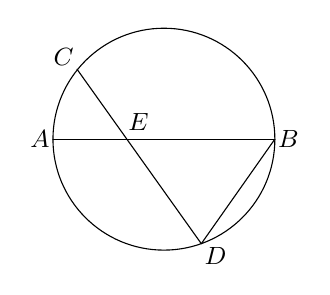
\begin{tikzpicture}[line cap=round,line join=round,font=\small]
\draw (0,0) circle (1.409);
\draw (-1.409,0)--(1.409,0);
\draw (-1.103,0.888)--(0.475,-1.327);
\draw (1.409,0)--(0.475,-1.327);
\node[above left,inner sep=1pt] at (-1.103,0.888) {$C$};
\node[left,inner sep=1pt] at (-1.409,0) {$A$};
\node at (-0.324,0.220) {$E$};
\node[right,inner sep=1pt] at (1.409,0) {$B$};
\node[below right,inner sep=1pt] at (0.475,-1.327) {$D$};
\end{tikzpicture}
\end{center}
\nopagebreak[4]
\end{question}
\begin{question}
\gkti{14}已知函数

\nopagebreak[4]
\[
f(x)=\begin{cases}
x^{2}+(4a-3)x+3a, & x<0,\\
\log_{a}(x+1)+1, & x\geqslant 0,
\end{cases}
\]

（\(a>0\) 且 \(a\neq 1\)）在 \(\mathbf{R}\) 上单调递减，且关于 \(x\) 的方程 \(|f(x)|=2-\dfrac{x}{3}\) 恰有两个不相等的实数解，则 \(a\) 的取值范围是 \(\underline{\qquad}\)。

\end{question}
\gkpart{三、解答题}

\begin{question}
\gkti{15}在 \(\triangle ABC\) 中，内角 \(A,B,C\) 所对应的边分别为 \(a,b,c\)。已知 \(a\sin 2B=\sqrt{3}b\sin A\)。

（1） 求 \(B\)；

（2） 若 \(\cos A=\dfrac{1}{3}\)，求 \(\sin C\) 的值。

\Needspace{0.4\textheight}
\end{question}
\begin{question}
\gkti{16}某化肥厂生产甲、乙两种混合肥料，需要 \(A,B,C\) 三种主要原料。生产 \(1\) 车皮甲种肥料和生产 \(1\) 车皮乙种肥料所需三种原料的吨数如下表所示：
\nopagebreak[4]
\begin{center}% 第 16 题原料用量表：按固定源 PDF 矢量路径换算（1 pt → 0.03515 cm）；原点取表格左下（源页 (913.89, 512.81) pt），y 向上。
% 4 条横线（含上下外框）、5 条竖线；表头行高 30.63 pt 约为数据行 15.51 pt 的两倍；
% 角格 45° 斜线自左上至右下，右上「原料」（对应 A,B,C 三列）、左下「肥料」（对应甲、乙两行）。
% 列宽（自左至右）66.28 / 20.22 / 20.84 / 22.85 pt；列标 A,B,C 为数学斜体，数据 4/8/3/5/5/10 为正体数字。
\begin{tikzpicture}[line cap=round,line join=round,font=\small,x=0.03515cm,y=0.03515cm]
% 横线（4 条）
\draw (0,61.65)--(130.59,61.65);
\draw (0,31.02)--(130.59,31.02);
\draw (0,15.51)--(130.59,15.51);
\draw (0,0)--(130.59,0);
% 竖线（5 条）
\draw (0.20,0)--(0.20,61.65);
\draw (66.48,0)--(66.48,61.65);
\draw (86.70,0)--(86.70,61.65);
\draw (107.54,0)--(107.54,61.65);
\draw (130.39,0)--(130.39,61.65);
% 角格斜线（左上→右下）
\draw (0.40,61.45)--(66.29,31.22);
% 斜线表头两角文字
\node[anchor=base west,inner sep=0] at (39.32,50.87) {原料};
\node[anchor=base west,inner sep=0] at (6.38,35.76) {肥料};
% 表头列标与数据行（各列居中）
\node[anchor=base] at (76.59,43.71) {\(A\)};
\node[anchor=base] at (97.12,43.71) {\(B\)};
\node[anchor=base] at (118.97,43.71) {\(C\)};
\node[anchor=base] at (33.34,20.24) {甲};
\node[anchor=base] at (76.59,20.24) {\(4\)};
\node[anchor=base] at (97.12,20.24) {\(8\)};
\node[anchor=base] at (118.97,20.24) {\(3\)};
\node[anchor=base] at (33.34,4.73) {乙};
\node[anchor=base] at (76.59,4.73) {\(5\)};
\node[anchor=base] at (97.12,4.73) {\(5\)};
\node[anchor=base] at (118.97,4.73) {\(10\)};
\end{tikzpicture}
\end{center}
\nopagebreak[4]
现有 \(A\) 种原料 \(200\) 吨，\(B\) 种原料 \(360\) 吨，\(C\) 种原料 \(300\) 吨，在此基础上生产甲乙两种肥料。已知生产 \(1\) 车皮甲种肥料，产生的利润为 \(2\) 万元；生产 \(1\) 车皮乙种肥料，产生的利润为 \(3\) 万元。分别用 \(x\)、\(y\) 表示生产甲、乙两种肥料的车皮数。

（1） 用 \(x,y\) 列出满足生产条件的数学关系式，并画出相应的平面区域；

（2） 问分别生产甲、乙两种肥料各多少车皮，能够产生最大的利润？并求出此最大利润。

\Needspace{0.4\textheight}
\end{question}
\begin{question}
\gkti{17}如图，四边形 \(ABCD\) 是平行四边形，平面 \(AED\perp\) 平面 \(ABCD\)，\(EF\parallel AB\)，\(AB=2\)，\(BC=EF=1\)，\(AE=\sqrt{6}\)，\(DE=3\)，\(\angle BAD=60^{\circ}\)，\(G\) 为 \(BC\) 的中点。
\nopagebreak[4]
\begin{center}% 第 17 题多面体（平行四边形 ABCD 上立平面 AED，含 F、E 与 BC 中点 G）：
% 按固定源 PDF 矢量路径端点换算（1 pt → 0.03515 cm）；原点取 C 点，y 向上。
% 源页顶点 pt：E(391.63,174.74)、F(334.74,174.74)、A(344.37,320.41)、B(230.60,320.41)、
% C(184.85,337.27)、D(298.62,337.27)、G(207.73,328.84)（G 为 BC 中点，坐标精确吻合）。
% 实线 6 条：EF、FC、CD、DA、DE、AE；虚线 6 条：CB、BA、BD、GF、BF、BE。先画虚线后画实线。
% 注：该图为示意，不按题设比例（∠BAD 实测约 20°、AB:BC 实测约 2.33:1），照源描摹，不按数值重定比例。
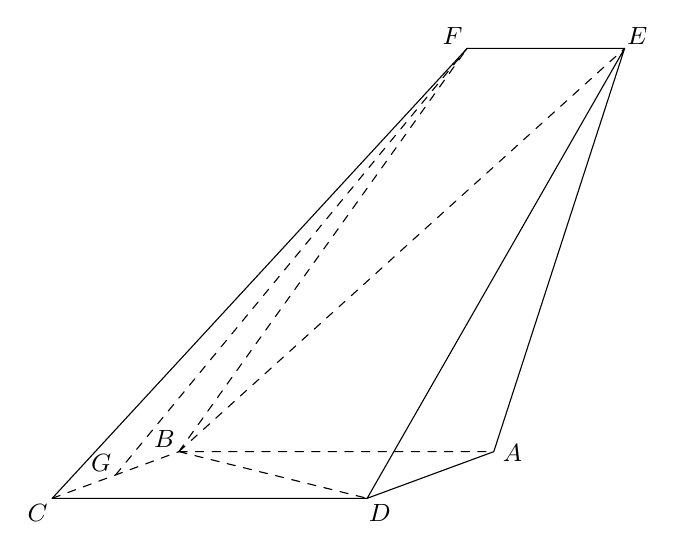
\begin{tikzpicture}[line cap=round,line join=round,font=\small,x=0.03515cm,y=0.03515cm]
\coordinate (E) at (206.78,162.53);
\coordinate (F) at (149.89,162.53);
\coordinate (A) at (159.52,16.86);
\coordinate (B) at (45.75,16.86);
\coordinate (C) at (0,0);
\coordinate (D) at (113.77,0);
\coordinate (G) at (22.88,8.43);
% 虚线先画（标签用 inner sep=0 + 源字形左端/基线显式坐标：TikZ 节点默认 inner sep
% 0.3333em 会把字形右移约 3pt，令 B/G 贴入顶点虚线簇；本图经 400 dpi 隔离探头
% 8-连通域验证 7 字母均为独立分量）
\draw[dashed] (C)--(B);
\draw[dashed] (B)--(A) (B)--(D) (G)--(F) (B)--(F) (B)--(E);
% 实线后画
\draw (E)--(F) (F)--(C) (C)--(D) (D)--(A) (D)--(E) (A)--(E);
% 标注（显式坐标：源字形左端与基线换算；不并入线段）
\node[anchor=base west,inner sep=0] at (140.86,163.87) {$F$};
\node[anchor=base west,inner sep=0] at (207.53,163.87) {$E$};
\node[anchor=base west,inner sep=0] at (162.56,13.27) {$A$};
\node[anchor=base west,inner sep=0] at (36.58,18.20) {$B$};
\node[anchor=base west,inner sep=0] at (13.82,9.77) {$G$};
\node[anchor=base west,inner sep=0] at (-9.06,-8.52) {$C$};
\node[anchor=base west,inner sep=0] at (114.21,-8.52) {$D$};
\end{tikzpicture}
\end{center}
\nopagebreak[4]
（1） 求证：\(FG\parallel\) 平面 \(BED\)；

（2） 求证：平面 \(BED\perp\) 平面 \(AED\)；

（3） 求直线 \(EF\) 与平面 \(BED\) 所成角的正弦值。

\end{question}
\begin{question}
\gkti{18}已知 \(\{a_{n}\}\) 是等比数列，前 \(n\) 项和为 \(S_{n}\)（\(n\in\mathbf{N}^{*}\)），且 \(\dfrac{1}{a_{1}}-\dfrac{1}{a_{2}}=\dfrac{2}{a_{3}}\)，\(S_{6}=63\)。

（1） 求数列 \(\{a_{n}\}\) 的通项公式；

（2） 若对任意的 \(n\in\mathbf{N}^{*}\)，\(b_{n}\) 是 \(\log_{2}a_{n}\) 和 \(\log_{2}a_{n+1}\) 的等差中项，求数列 \(\{(-1)^{n}b_{n}^{2}\}\) 的前 \(2n\) 项和。

\end{question}
\begin{question}
\gkti{19}设椭圆 \(\dfrac{x^{2}}{a^{2}}+\dfrac{y^{2}}{3}=1\)（\(a>\sqrt{3}\)）的右焦点为 \(F\)，右顶点为 \(A\)。已知 \(\dfrac{1}{|OF|}+\dfrac{1}{|OA|}=\dfrac{3e}{|FA|}\)，其中 \(O\) 为原点，\(e\) 为椭圆的离心率。

（1） 求椭圆的方程；

（2） 设过点 \(A\) 的直线 \(l\) 与椭圆交于点 \(B\)（\(B\) 不在 \(x\) 轴上），垂直于 \(l\) 的直线与 \(l\) 交于点 \(M\)，与 \(y\) 轴交于点 \(H\)。若 \(BF\perp HF\)，且 \(\angle MOA=\angle MAO\)，求直线 \(l\) 的斜率。

\end{question}
\begin{question}
\gkti{20}设函数 \(f(x)=x^{3}-ax-b\)，\(x\in\mathbf{R}\)，其中 \(a,b\in\mathbf{R}\)。

（1） 求 \(f(x)\) 的单调区间；

（2） 若 \(f(x)\) 存在极值点 \(x_{0}\)，且 \(f(x_{1})=f(x_{0})\)，其中 \(x_{1}\neq x_{0}\)，求证：\(x_{1}+2x_{0}=0\)；

（3） 设 \(a>0\)，函数 \(g(x)=|f(x)|\)，求证：\(g(x)\) 在区间 \([-1,1]\) 上的最大值不小于 \(\dfrac{1}{4}\)。

\end{question}